% Распределение вычислительной нагрузки между узлами гетерогенного вычислительного кластера.
\subsection{Распределение вычислительной нагрузки между узлами гетерогенного вычислительного кластера}

Рассмотрим фиксированную декомпозированную расчетную задача.
Это могут быть вычисления, выполняемые на блочно-структурированной расчетной сетке, либо на неструктурированной сетке, разбитой на домены.
При распределении частей расчетной задачи между вычислителями суперкомпьютерного кластера для уменьшения времени выполнения задачи важно учитывать характеристики самого кластера, к которым относится производительность вычислителей и скорость обмена данными между ними.
В этом разделе приводится описание эвристического алгоритма распределения вычислительной нагрузки на вычислительном кластере с учетом геометрии расчетной задачи и характеристик кластера.

\subsubsection{Постановка задачи}

\begin{definition}
Графом вычислительного кластера назовем граф $H = (V_H, E_H)$.
Узлы этого графа соответствуют отдельным вычислителям кластера (одному процессору или сопроцессору), а ребра -- логическим соединениям между вычислителями (то есть возможностью обмена данными).
\end{definition}

Так как между любыми двумя вычислителями возможен обмен данными, то граф $H$ является полным (и даже является псевдографом, так как содержит все возможные петли).
Введем на графе $H$ две весовые функции.
Первая функция $f: V_H \rightarrow \mathbb{R}_{> 0}$ каждому узлу графа ставит в соответствие скорость работы соответствующего вычислителя, то есть количество расчетных данных, которые могут быть обработаны на нем за одну условную единицу времени (для разных вычислительных задач функции могут различаться).
Вторая функция $l: E_H \rightarrow \mathbb{R}_{> 0}$ несет смысл скорости обмена данными между вычислителями, она показывает количество данных, которые могут быть переданы между соответствующими вычислителями за одну условную единицу времени.

\begin{definition}
Графом расчетной задачи назовем граф $G = (V_G, E_G)$, который отражает особенности декомпозиции расчетной области (это может быть граф блочно-структурированной расчетной сетки или граф доменов неструктурированной сетки).
Узлы этого графа соответствуют компактно расположенным в пространстве множествам данных, каждое из которых обрабатывается одним вычислителем.
Ребра графа соответствуют потокам данных между разными частями задачи.
\end{definition}

На графе $G$ также вводятся две весовые функции.
Первая функция $w: V_G \rightarrow \mathbb{R}_{> 0}$ имеет значение объема вычислительных данных, обрабатываемых в соответствующей части задачи.
Вторая функция $i: E_G \rightarrow \mathbb{R}_{> 0}$ отражает объем данных, пересылаемых между частями задачи при межпроцессном обмене.
Значения всех четырех функций $f$, $l$, $w$, $i$ измеряются в одних и тех же единицах (это могут быть ячейки расчетной сетки, количество байтов или вещественных значений).

Расчет задачи состоит из двух чередующихся фаз: проведение итерации расчета и выполнение межпроцессных обменов данными.
Будем считать, что эти фазы не перемешиваются для отдельных частей задачи (хотя возможно выполнять расчеты для одной части задачи и одновременно проводить межпроцессные обмены для другой ее части).
Требуется таким образом распределить задачу между вычислителями кластера, чтобы суммарное время одной итерации расчета и одной итерации межпроцессных обменов было минимально.
Распределение задачи между вычислителями кластера определяется функцией $\gamma: V_G \rightarrow V_H$.

Время выполнения одной итерации вычислений определяется по самому загруженному вычислителю:
\begin{equation}
	t_1^{max} = \max_{v_H \in V_H}{\left( \frac{1}{f(v_H)} \sum_{\substack{v_G \in V_G \\ \gamma(v_G) = v_H}}{w(v_G)} \right)}
\end{equation}

Аналогично время выполнения одной итерации межпроцессных обменов определяется по самому загруженному каналу обмена:
\begin{equation}
	t_2^{max} = \max_{e_H \in E_H}{\left( \frac{1}{l(e_H)} \sum_{\substack{e_G = (u_G, v_G) \in E_G \\ (\gamma(u_G), \gamma(v_G)) = e_H}}{e(e_G)} \right)}
\end{equation}

Таким образом, задача поиска оптимального распределения задачи по вычислителям кластера сводится к поиску функции $\gamma$, минимизирующей значение функционала $t^{max}(\gamma) = t_1^{max}(\gamma) + t_2^{max}(\gamma)$.
Так как каждый элемент из множества $V_G$ может быть отнесен к любому вычислителю, то общее количество всех функций распределения равно $|V_H|^{|V_G|}$.

Можно рассматривать частные случае задачи распределения вычислительной нагрузки.
Для вычислительных задач с малой долей мепроцессных обменов можно ограничиться минимизацией функционала $t^{max}(\gamma) = t_1^{max}(\gamma)$.
Также можно рассматривать задачу распределения для гомогенного кластера, для которого функции $f$ и $l$ являются константами. Минимизируемый функционал в этом случает принимает следующий вид:
\begin{equation}
	t^{max}(\gamma) =
		\frac{1}{f} \max_{v_H \in V_H}{\left( \sum_{\substack{v_G \in V_G \\ \gamma(v_G) = v_H}}{w(v_G)} \right)} + 
		\frac{1}{l} \max_{e_H \in E_H}{\left( \sum_{\substack{e_G = (u_G, v_G) \in E_G \\ (\gamma(u_G), \gamma(v_G)) = e_H}}{i(e_G)} \right)}
\end{equation}

Рассмотрим эвристический алгоритм поиска приближенного решения поставленной задачи, который учитывает весовые функции графов задачи и вычислительного кластера, а также геометрию расчетной области задачи.

\subsubsection{Описание алгоритма}

Одной из особенностей вычислительного кластера является то, что скорость обмена данными между двумя частями задачи, обрабатываемыми одним вычислителем, существенно выше, чем скорость обмена данными между двумя частями задачи, обрабатываемыми двумя разными вычислителями.
Интуитивно понятно, что задача должна распределяться между узлами вычислительного кластера таким образом, чтобы расположенные рядом части задачи попадали на один вычислитель.
В идеале граф $G$ задачи должен быть разбит на $|V_H|$ связных партиций, каждая из которых обрабатывается своим вычислителем, причем вес партиции (суммарный вес частей задачи, входящих в партицию), должен быть пропорционален весу соответствующего вычислителя.

Каждому узлу графа $G$ поставлена в соответствие точка трехмерного пространства (центр соответствующей части расчетной задачи). 
С использованием данных точек формировать партиции можно по геометрическому принципу. Для этого сначала нужно выполнить первую фазу алгоритма -- определить базовые точки, вокруг которых в дальнейшем будут формироваться партиции.
Базовые точки должны быть распределены по объему расчетной области задачи таким образом, чтобы веса сформированных впоследствии партиций были пропорциональны весам вычислителей.
Будем считать, что все ячейки расчетной сетки, используемой в задаче, имеют примерно равные размеры.
Это означает, что нет заметных сгущений и разряжений сетки.
В условии нашего допущения объем области, занимаемой партицией, будет пропорционален ее весу.
Таким образом, задача определения базовых точек сводится к следующей: требуется в данной области пространства определить такое множество точек, чтобы объемы окрестностей, окружающих эти точки, были пропорциональны весам вершин графа $H$.
При этом окрестность точки строго не определяется.
Главное, чтобы окрестность содержала саму точку и имела интуитивно компактную форму.

Добиться определения базовых точек можно с помощью простого итерационного алгоритма с имитацией взаимного отталкивания точек друг от друга.
Обозначим область расчетной задачи через $\Omega$.
На первом шаге расположим $|V_H|$ точек (будем обозначать их с помощью соответствующих радиус-векторов) случайным образом внутри области $\Omega$.
Каждой базовой точке поставим в соответствие конкретную вершину графа $H$.
Таким образом, каждая точка $\overline{p}(v_H)$ будет иметь вес $f(v_H)$.
Далее на каждом шаге будем моделировать силу взаимного отталкивания между двумя точками $\overline{p}(v_1)$ и $\overline{p}(v_2)$ по закону
\begin{equation}
	F(\overline{p}(v_1), \overline{p}(v_2)) = \frac{f(v_1) f(v_2)}{|\overline{p}(v_1) - \overline{p}(v_2)|^2}
\end{equation}

После этого будем корректировать положение каждой точки под действием суммарной силы отталкивания от всех остальных точек.
Кроме того, суммарную силу нужно дополнить корректирующей силой отталкивания от границ области $\Omega$, иначе все точки будут располагаться на этой границе.
Алгоритм заканчивает свою работу, когда положение точек стабилизируется, что говорит об уравнивании всех моделируемых сил отталкивания.

\begin{figure}[ht]
	\centering
		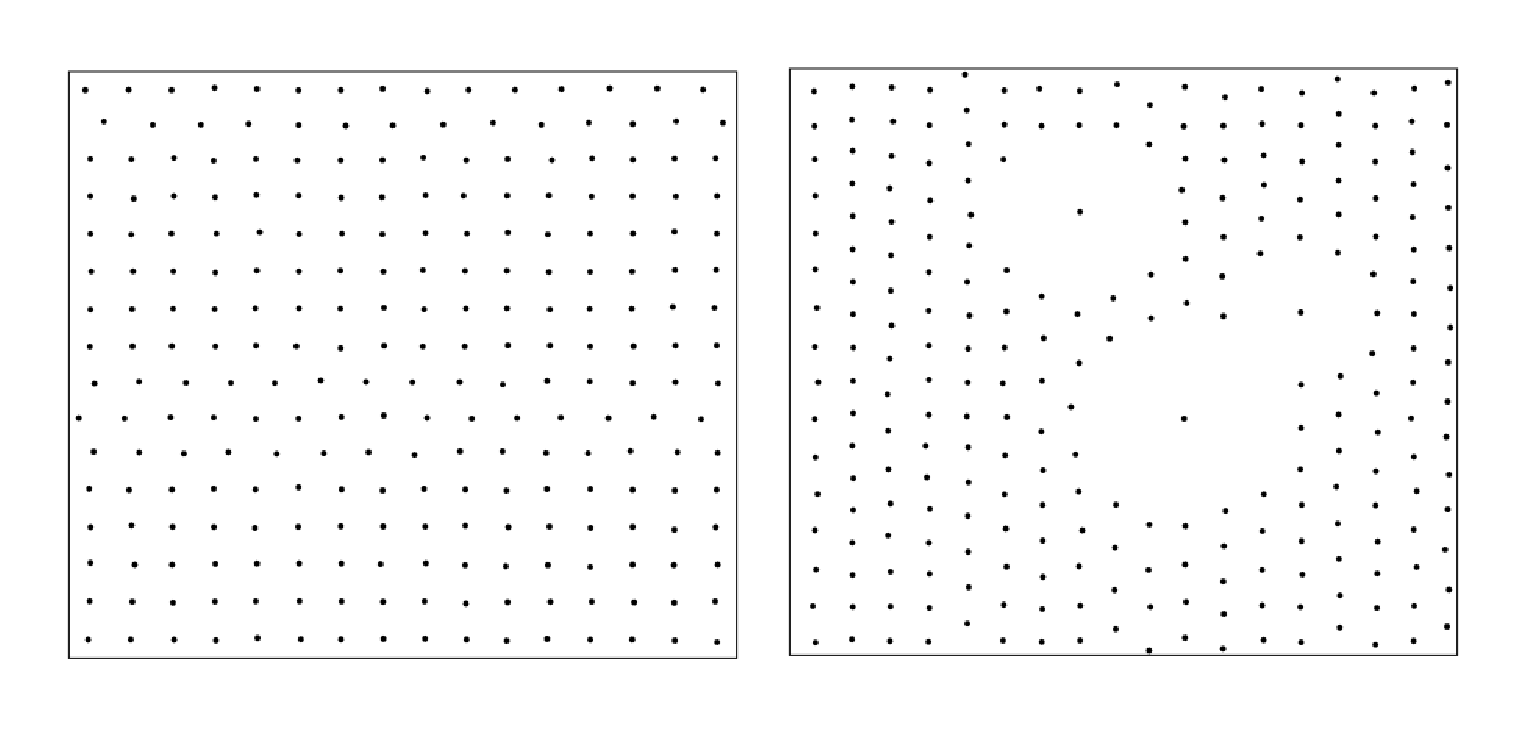
\includegraphics[width=0.8\textwidth]{./pics/text_2_getero/rvp.pdf}
	\caption{Иллюстрация работы алгоритма определения базовых точек.}
	\label{fig:text_2_getero_rvp}
\end{figure}

На рис.~\ref{fig:text_2_getero_rvp} показана иллюстрация работы алгоритма определения базовых точек внутри квадратной области в двумерном случае.
На рисунке слева все точки имеют одинаковые веса, на рисунке справа выделены три точки, имеющие случайные веса значительно выше среднего значения.
После определения базовых точек можно переходить ко второй фазе алгоритма -- определение (наращивание) партиций вокруг базовых точек.
На каждом шаге наращивания партиций будем выбирать партицию с минимальным значением
\begin{equation}
	\frac{1}{f(v_H)} \sum_{\substack{v_G \in V_G \\ \gamma(v_G) = v_H}}{w(v_G)},
\end{equation}

характеризующим время обработки данных этой партиции на одной итерации расчетов, и добавлять к ней новую вершину из $V_G$.
Если на текущем шаге рассматриваемая партиция пуста, то добавим к ней вершину из $V_G$, расположенную ближе всех к базовой точке $\overline{p}(v_H)$.
Если рассматриваемая партиция уже содержит точки, то рассмотрим ее окрестность.

\begin{definition}
Окрестностью партиции $\delta(v_H)$ назовем множество не входящих в нее (и ни в какую другую партицию) вершин графа $G$, соединенных ребром хотя бы с одной вершиной из этой партиции.
\end{definition}

Выберем из этой окрестности вершину $v$ с максимальным показателем предпочтения $q(v)$, который определяется по следующей формуле:
\begin{equation}\label{eqn:text_2_getero_q}
	q(v) = \frac{w(v)}{f(v_H)} +
		\left( \sum_{\substack{e = (u, v) \in E_G \\ \gamma(u) = v_H}}{i(e)} \right) \cdot
		\left( \frac{\sum_{\substack{e_H = (u', v') \in E_H \\ u' \ne v'}}{l(e_H)}}{|E_H| - |V_H|} \right)^{-1}
\end{equation}

Первое слагаемое в \eqref{eqn:text_2_getero_q} отражает скорость обработки данных из части задачи, соответствующей вершине $v$, на вычислителе $v_H$.
Второе слагаемое отражает время межпроцессных обменов, которое удастся сократить после добавление в партицию вершины $v$ (при этом в качестве скорости обменов берется среднее значение функции $l$ по всем вершинам графа $H$ за исключением петель).

\begin{figure}[ht]
	\centering
		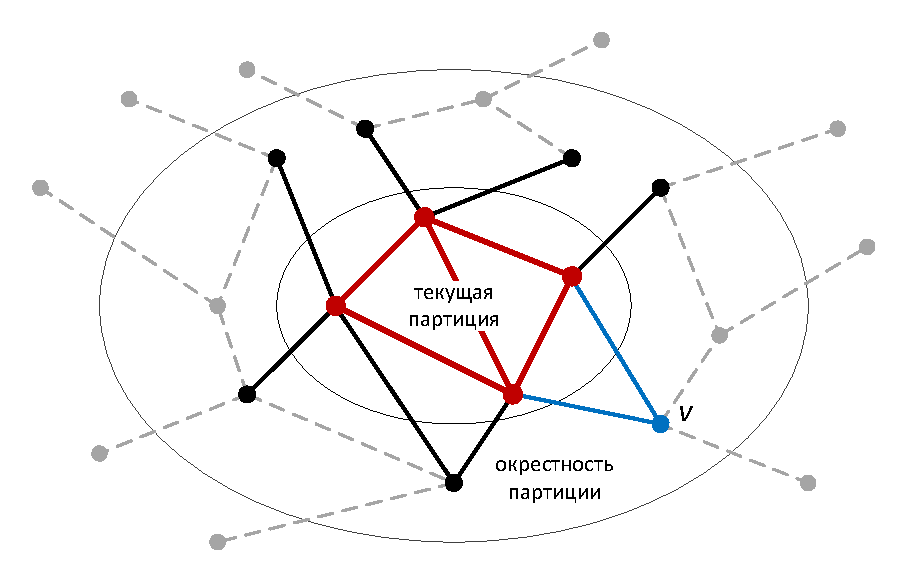
\includegraphics[width=0.8\textwidth]{./pics/text_2_getero/partition.pdf}
	\caption{Добавление новой вершины в партицию.}
	\label{fig:text_2_getero_partition}
\end{figure}

На рис.~\ref{fig:text_2_getero_partition} приведена иллюстрация расширения текущей партиции (отмечено красным) за счет добавления новой вершины ($v$).
При этом ребра, отмеченные синим цветом становятся внутренними ребрами партиции, что гарантирует ускорение обмена данными по этим ребрам.

Так как количество вершин в графе $G$ конечно, а на каждом шаге алгоритма в некоторую партицию добавляется одна вершина, то алгоритм заканчивает свою работу, когда все вершины распределены по партициям.

На шаге расширения партиции возможна такая ситуация, когда вся окрестность текущей партиции уже распределена по соседним партициям.
Такое возможно на последних шагах распределения, когда остается малое количество нераспределенных частей задачи.
В этом случае партицию можно расширить просто ближайшей свободной вершиной графа $G$.
Это приводит к тому, что в распределении оказываются отдельные вершины графа $G$, принадлежащие одной партиции, полностью окруженные вершинами из других партиций.
Для корректировки таких неэффективных с точки зрения обмена данными аномалий выполняется третья фаза алгоритма -- захват партициями внутренних точек, на которой партиция может поглотить небольшие анклавы вершин графа $G$.

\subsubsection{Результат работы}

Для анализа эффективности работы описанного алгоритма рассматривалась модельная задача, двумерная квадратная расчетная область которой равномерно разбита близкие по размеру части.
В качестве расчетного кластера рассматривались гомогенный и гетерогенный кластеры, содержащие 8 вычислителей.

\begin{figure}[ht]
	\centering
		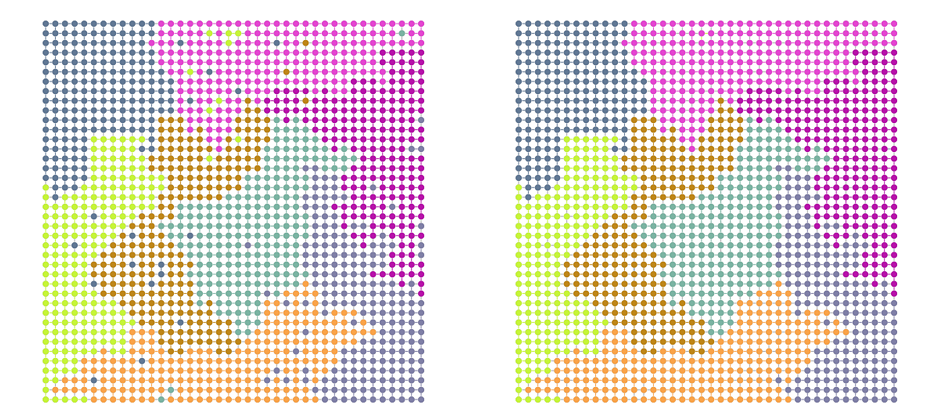
\includegraphics[width=0.8\textwidth]{./pics/text_2_getero/res1small.png}
	\caption{Результат применения алгоритма для распределения вычислительной нагрузки между вычислительного гомогенного кластера.}
	\label{fig:text_2_getero_res1}
\end{figure}

На рис.~\ref{fig:text_2_getero_res1} проиллюстрирована работа алгоритма распределения вычислительной нагрузки для модельной задачи между 8 вычислителями гомогенного кластера (то есть все вычислители идентичны).
Слева представлены результаты после второй фазы алгоритма, при этом наблюдается некоторое перемешивание партиций.
Справа показаны результаты после третьей фазы алгоритма, на которой корректируется связность партиций путем поглощения отдельных узлов графа $G$, попавших не в свою партицию.

\begin{figure}[ht]
	\centering
	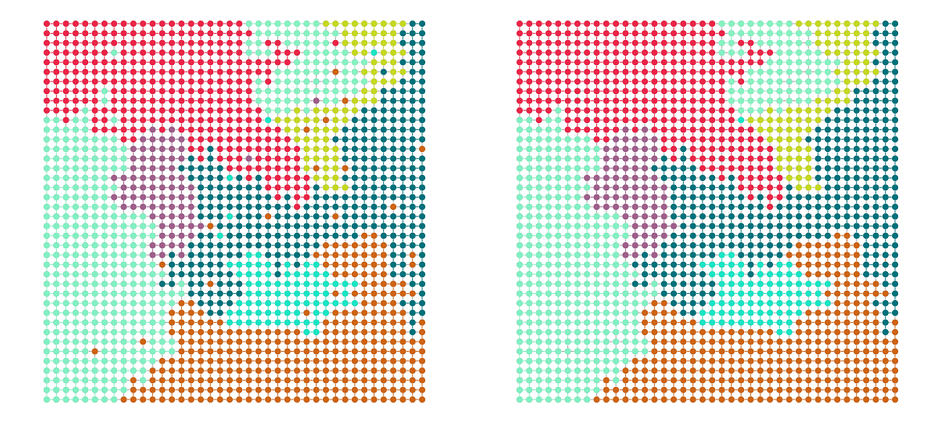
\includegraphics[width=0.8\textwidth]{./pics/text_2_getero/res2small.png}
	\caption{Результат применения алгоритма распределения вычислительной нагрузки между вычислителями гетерогенного кластера.}
	\label{fig:text_2_getero_res2}
\end{figure}

На рис.~\ref{fig:text_2_getero_res2} показаны аналогичные результаты работы алгоритма для гетерогенного кластера, состоящего из узлов двух типов, отличающихся по производительности друг от друга в 4 раза.
На иллюстрациях видна разница в размерах партиций, отнесенных к тому или иному типу вычислителя.

Из рис.~\ref{fig:text_2_getero_res1} и рис.~\ref{fig:text_2_getero_res2} видно, что получившиеся партиции имеют довольно протяженные изломанные границы, что негативно влияет на скорость межпроцессных обменов.
Для их сокращения требуется проведение дополнительной фазы алгоритма, состоящей в выравнивании границ.

Для оценки эффективности алгоритма кроме характеристики времени исполнения одной вычислительной итерации и одной итерации межпроцессных обменов $t^{max}(\gamma)$ расчитывалась аналогичная характеристика
\begin{equation}
	t^{max}(\gamma) =
		\frac{1}{f} \min_{v_H \in V_H}{\left( \sum_{\substack{v_G \in V_G \\ \gamma(v_G) = v_H}}{w(v_G)} \right)} + 
		\frac{1}{l} \min_{e_H \in E_H}{\left( \sum_{\substack{e_G = (u_G, v_G) \in E_G \\ (\gamma(u_G), \gamma(v_G)) = e_H}}{i(e_G)} \right)}
\end{equation}

Разность этих двух значений отражает неэффективность распределения, связанную с простоем вычислительных ресурсов.

\begin{figure}[H]
	\centering
		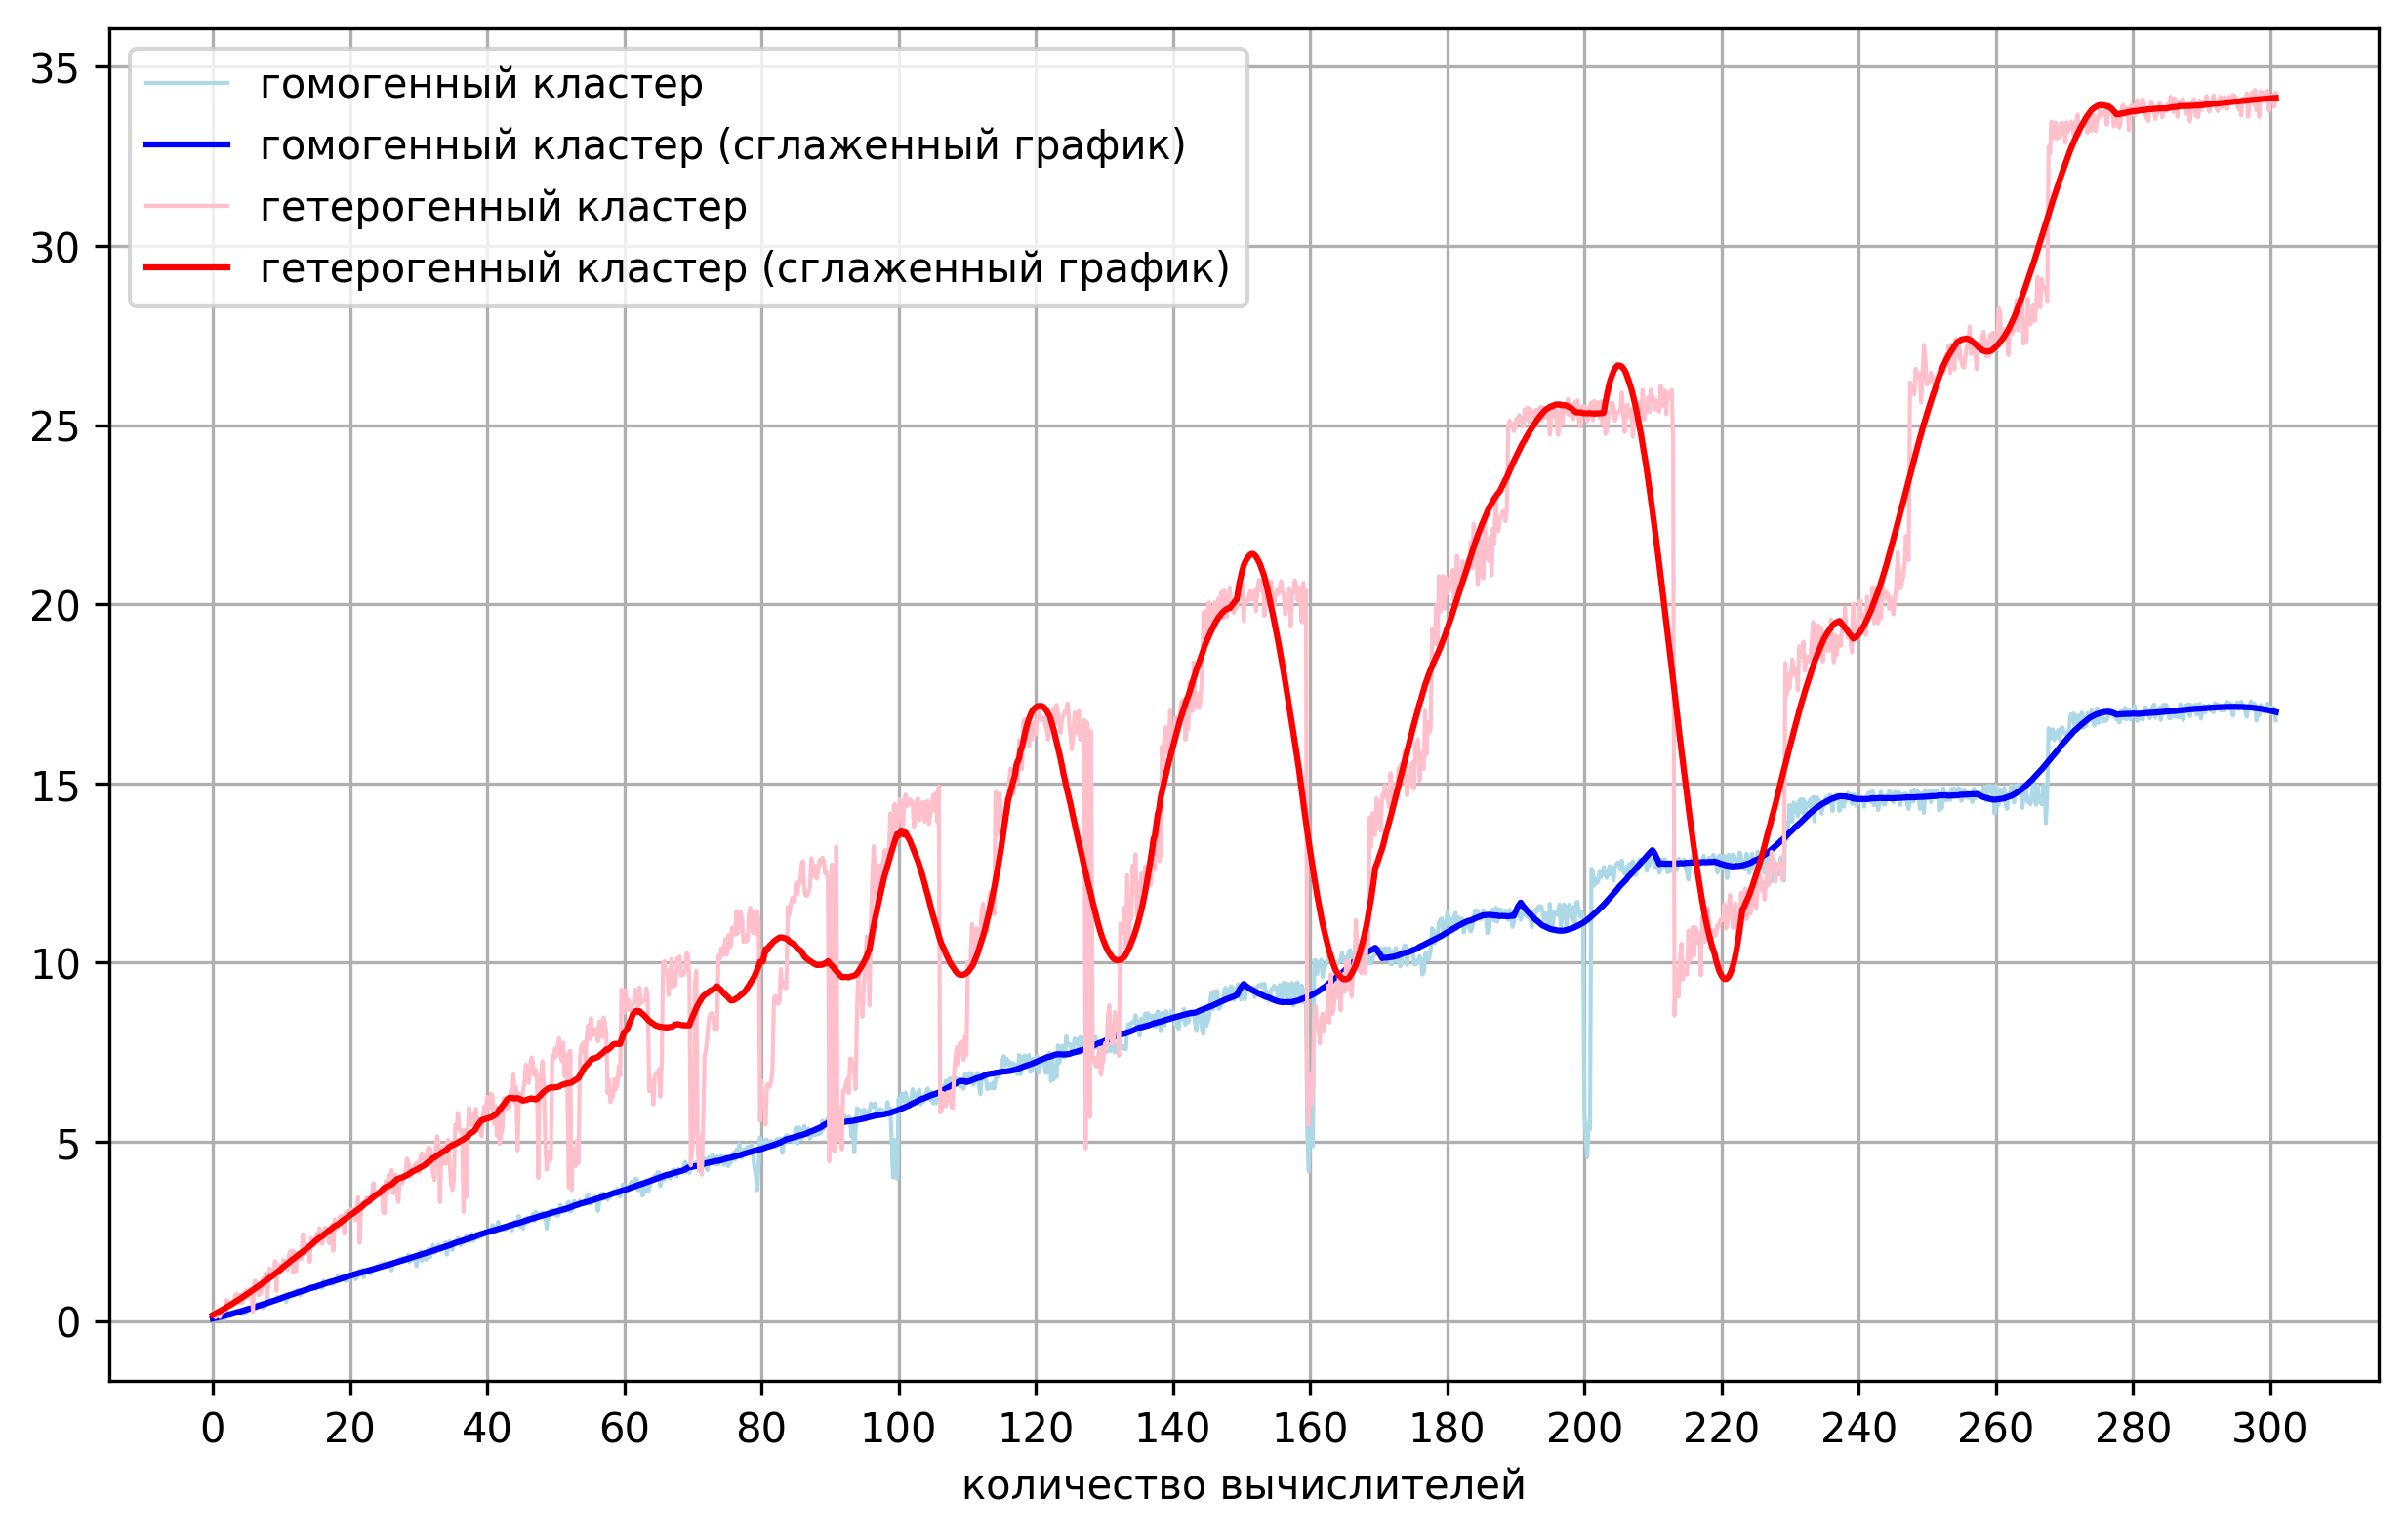
\includegraphics[width=0.8\textwidth]{./pics/text_2_getero/chart2.png}
	\caption{Зависимость показателя эффективности распределения задачи между узлами гомогенного и гетерогенного вычислительных кластеров (по горизонтали отложено количество вычислителей, по вертикали -- значение $\frac{t^{max} - t^{min}}{t^{min}} \cdot 100\%$.}
	\label{fig:text_2_getero_chart}
\end{figure}

Для модельной задачи были проведены эксперименты по распределению графа задачи на узлы гомогенного и гетерогенного кластера при изменении количества вычислителей от 2 до 300.
На рис.~\ref{fig:text_2_getero_chart} представлены полученные зависимости.
Видно, что для обоих видов кластеров при увеличении количества вычислителей наблюдается линейная тенденция к снижению эффективности распределения, но в случае гетерогенного кластера эффективность распределения ниже и зависимость от количества узлов в этом случае более сложная.
